\documentclass[11pt]{beamer}
\usepackage[T1]{fontenc}
\usepackage[utf8]{inputenc}
\usepackage{lmodern}
\usepackage[francais]{babel}

\usepackage{textpos}

\usepackage{graphicx}
\usepackage{tabularx}
\usepackage{lastpage}
\usepackage[top=2.75cm, bottom=3cm, left=2cm, right=2cm]{geometry}
\usepackage[colorlinks=true, urlcolor=blue, linkcolor=black, citecolor=black]{hyperref}
\usepackage{calc}
\usepackage{amsmath} % equation align
\usepackage{amsfonts}
\usepackage{amssymb}
\usepackage{fancyhdr}
\usepackage[format=hang, width=.8\textwidth, labelfont=sc]{caption}
\usepackage[format=hang, width=.8\textwidth, labelfont=normalfont]{subcaption}
% \usepackage[labelformat=empty]{caption} % no label before caption
\usepackage{verbatim}

% paragraph and subparagraph as level 4 and 5 sections
\usepackage{titlesec}
\usepackage{titletoc}
\setcounter{secnumdepth}{5}
\setcounter{tocdepth}{5}
\titleformat{\paragraph} [hang] {\normalfont\normalsize\bfseries} {\theparagraph} {1em} {}
\titleformat{\subparagraph} [hang] {\normalfont\normalsize\bfseries} {\thesubparagraph} {1em} {}

% lists config
\usepackage{enumitem}
\setlist[itemize]{label=-}

% replace no-break space
\DeclareUnicodeCharacter{00A0}{ }

% header & footer
\pagestyle{fancy}
\fancyhf{}
\setlength{\headheight}{14pt}
\lhead{{\small \ititle}}
\rhead{{\small \isubtitle}}
\lfoot{}
\rfoot{\hrule\vspace{.1cm}\thepage /\pageref*{LastPage}}


% title info
% \title{Projet IA04 - NF28}
% \subtitle{Colladia, éditeur de diagramme collaboratif}
\author{Jean Vintache\\Florian Impellettieri\\Charles Menier\\Marouane Hammi\\Adrien Jacquet}
% \author[short]{author}
\date{\today}
% \titlegraphic{\vspace{-2.25cm}\includegraphics[height=4cm]{img/gliese581_2.jpg}}
\logo{ % logo on titlepage only
	\ifnum \insertpagenumber=1
		\vspace{-0.2cm}
\includegraphics[scale=0.1]{img/utc-logo.jpg}
	\fi
}

% \AtBeginSection[]
% {
%    \begin{frame}%[allowframebreaks] % multiple frames
% 	   \frametitle{Sommaire}
% 	   \tableofcontents[currentsection]
%    \end{frame}
% }


\begin{document}
\title{
		\hspace*{-.55cm}
		\begin{tikzpicture}
		\node [inner sep=0pt] at (0,0) {
\includegraphics[width=\textwidth]{img/colladia-banner}};
		\draw [white, rounded corners=\ClipSep, line width=\ClipSep] 
				(current bounding box.north west) -- 
				(current bounding box.north east) --
				(current bounding box.south east) --
				(current bounding box.south west) -- cycle
				;
		\end{tikzpicture}
}

\small
\begin{frame}
	\vspace{-0.75cm}
	\titlepage
\end{frame}

%\begin{frame}%[allowframebreaks] % multiple frames
%	\frametitle{Sommaire}
%	\tableofcontents
%\end{frame}

\section{Présentation du projet}
\begin{frame}
	\frametitle{\currentname}
	\begin{itemize}
		\item Éditeur de diagramme collaboratif pour Android
		\\~\\
		\item Client (Contexte NF28)
		\begin{itemize}
		  \item Java Android natif
			\item Communication avec le serveur via des requêtes HTTP REST
			\item Synchronisation par des requêtes GET périodiques
		\end{itemize}
		~\\
		\item Serveur (Contexte IA04)
		\begin{itemize}
			\item Système multi-agent JADE
			\item Sauvegarde et synchronise l'état des diagrammes entre les différents clients
			\item Implémente des fonctions d'ajout, modification, suppression et auto-positionnement d'éléments
		\end{itemize}
	\end{itemize}
\end{frame}

\section{Organisation des vues}
\begin{frame}
	\frametitle{\currentname}
  
%	\begin{center}
%		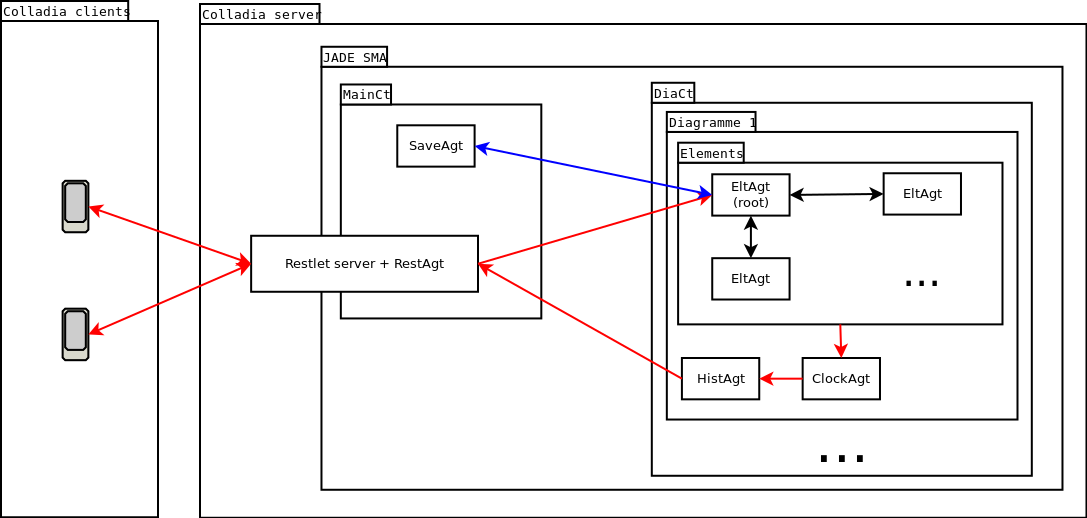
\includegraphics[width=\textwidth]{img/general_server}
%	\end{center}
\end{frame}

\section{Fonctionnalités}
\begin{frame}
	\frametitle{\currentname}
  
%	\begin{center}
%		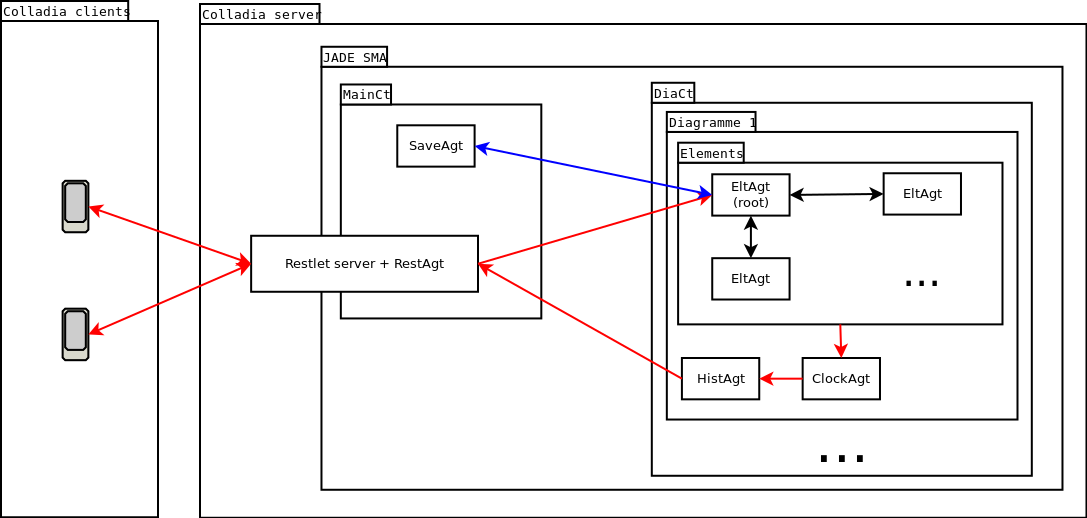
\includegraphics[width=\textwidth]{img/general_server}
%	\end{center}
\end{frame}

\section{Vidéo démo}
\begin{frame}
	\frametitle{\currentname}
  
	\begin{center}
    \url{https://www.youtube.com/watch?v=ffRjMP_Aqt0}
	\end{center}
\end{frame}

\end{document}
